\documentclass[12pt, twoside]{article}
% \documentclass[12pt, twoside]{article}
\usepackage[letterpaper, margin=1in, headsep=0.2in]{geometry}
\setlength{\headheight}{0.6in}
%\usepackage[english]{babel}
\usepackage[utf8]{inputenc}
\usepackage{microtype}
\usepackage{amsmath}
\usepackage{amssymb}
%\usepackage{amsfonts}
\usepackage[nomessages]{fp} %\FPeval{\var-name}{2*sin(pi/6)}
\usepackage{siunitx} %units in math. eg 20\milli\meter
\usepackage{yhmath} % for arcs, overparenth command
\usepackage{tikz} %graphics
\usetikzlibrary{quotes, angles, arrows, arrows.meta}
\usepackage{graphicx} %consider setting \graphicspath{{images/}}
\usepackage{parskip} %no paragraph indent
\usepackage{enumitem}
\usepackage{multicol}
\usepackage{venndiagram}

\usepackage{fancyhdr}
\pagestyle{fancy}
\fancyhf{}
\renewcommand{\headrulewidth}{0pt} % disable the underline of the header
\raggedbottom
\hfuzz=2mm %suppresses overfull box warnings

\usepackage{hyperref}
\usepackage{float}

\fancyhead[LE]{\thepage}
\fancyhead[RO]{\\ First and last name: \hspace{2.5cm} \,\\ Section: \hspace{2.5cm} \,}
\fancyhead[LO]{BECA/Huson/Precalculus: Sequences \\* 9 September 2024}

\begin{document}
\begin{itemize}
  \item[$\square$] I brought a calculator to class today.
\end{itemize}

\subsubsection*{1.3 Do Now: Area and length calculations}
\begin{enumerate}

\item What is the distance between $P$ and $Q$ on the number line? \par \smallskip
  \begin{tikzpicture}
    \draw [<->] (-2.5,0)--(6.5,0);
    \foreach \x in {-2,...,6} %2 leading for diff!=1
      \draw[shift={(\x,0)},color=black] (0pt,-3pt) -- (0pt,3pt) node[below=5pt]  {$\x$};
      \draw [fill] (2,0) circle [radius=0.05] node[above] {$P$};
      \draw [fill] (6,0) circle [radius=0.05] node[above] {$Q$};
  \end{tikzpicture} \hspace{2cm}
  $PQ=$

\item Points $A=4 \frac{1}{2}$ and $B=16 \frac{1}{4}$ are shown below. Find ${AB}$. \par \smallskip
\begin{tikzpicture}[scale=0.5]
  \draw [<->] (-1,0)--(21,0);
  \foreach \x in {0, 2,...,20} %2 leading for diff!=1
    \draw[shift={(\x,0)},color=black] (0pt,-6pt) -- (0pt,6pt) node[below=5pt]  {$\x$};
    \draw [fill] (4.5,0) circle [radius=0.1] node[above] {$A$};
    \draw [fill] (16.25,0) circle [radius=0.1] node[above] {$B$};
\end{tikzpicture}

\item What is the distance on the number line between the points $F$ and $G$? \par \smallskip
  \begin{tikzpicture}
    \draw [<->] (-2.5,0)--(6.5,0);
    \foreach \x in {-2,...,6} %2 leading for diff!=1
      \draw[shift={(\x,0)},color=black] (0pt,-3pt) -- (0pt,3pt) node[below=5pt]  {$\x$};
      \draw [thick] (1.25,0)--(5.5,0);
      \draw [fill] (1.25,0) circle [radius=0.05] node[above] {$F(1.25)$};
      \draw [fill] (5.5,0) circle [radius=0.05] node[above] {$G(5.50)$};
  \end{tikzpicture}

\item Find the area $A$ and perimeter $P$ of the shape shown below. Assume the grid is in inches.
  \begin{flushleft}
    \begin{tikzpicture}[scale=0.75]
      \draw[help lines] (-4,-4) grid (5,3);
      \draw[thick, -] (-3,-3)--(4,-3)--(4,2)--(2,2)--(-3,2)--cycle;
    \end{tikzpicture}
  \end{flushleft}

\item Find the area of a rectangle with length $l=3 \frac{1}{2}$ and width $w=5$. Use the formula for the area of a rectangle: $A = l \times w$
  \begin{flushright}
  \begin{tikzpicture}[scale=1.25]
    \draw[thick] (0,0)--(3,0)--(3,3.5)--(0,3.5)--cycle;
    \node at (3.5, 2){5};
    \node at (1.5, -0.3){$3 \frac{1}{2}$};
    \node at (1.5, 2){$A = ?$};
  \end{tikzpicture}
  \end{flushright}


\item Find the length of the base of a rectangle with area $A=22 \frac{1}{2}$ and height $h=5$, expressed as a fraction. Start with the form (use $b$ or $x$): \par \medskip
$A = b \times h = 22 \frac{1}{2}$
  \begin{flushright}
  \begin{tikzpicture}[scale=1.25]
    \draw[thick] (0,0)--(3,0)--(3,3.5)--(0,3.5)--cycle;
    \node at (3.5, 2){5};
    \node at (1.5, -0.3){$?$};
    \node at (1.5, 2){$A = 22 \frac{1}{2}$};
  \end{tikzpicture}
  \end{flushright}

\newpage

  
\item Find the area of $\triangle ABC$. The altitude $h$ of the triangle is $8$ centimeters and the base $AB=10 \frac{1}{2}$ cm. (diagram not to scale) \par
  \begin{tikzpicture}[scale=1]
    \draw[thick]
      (0,0)node[below]{$A$}--
      (6,0)node[below]{$B$}--
      (4,3)node[above]{$C$}--cycle;
   \draw[dashed] (4,0)--(4,3);
   \draw (4,0)++(0.3,0)--++(0,0.3)--+(-0.3,0);
   \node at (3.3,1.2){$h=8$};
   \node at (3,0)[below]{$10 \frac{1}{2}$ cm};
  \end{tikzpicture}

\item Find the length of the base of a triangle with area $A=35$ and height $h=10$. Start with the form (use $b$ or $x$): \par \medskip
  $A = \frac{1}{2} \times b \times h = 35$
  \begin{flushright}
  \begin{tikzpicture}[scale=1.25]
    \draw[thick] (0,0)--(3,0)--(2.5,3.5)--cycle;
    \draw[<->,dashed] (3.3,0)--(3.3,3.5);
    \node at (3.6,1.7){10};
    \node at (1.5,0.3){$b=?$};
    \node at (1.8,1.4){$A = 35$};
  \end{tikzpicture}
  \end{flushright}


\end{enumerate}
\end{document}